\documentclass[11pt,twoside,a4paper]{article}
% http://www-h.eng.cam.ac.uk/help/tpl/textprocessing/latex_maths+pix/node6.html symboles de math
% http://fr.wikibooks.org/wiki/Programmation_LaTeX Programmation latex (wikibook)
%=========================== En-Tete =================================
%--- Insertion de paquetages (optionnel) ---
\usepackage[french]{babel}   % pour dire que le texte est en fran{\'e}ais
\usepackage{a4}	             % pour la taille   
\usepackage[T1]{fontenc}     % pour les font postscript
\usepackage{epsfig}          % pour gerer les images
%\usepackage{psfig}
\usepackage{amsmath, amsthm} % tres bon mode mathematique
\usepackage{amsfonts,amssymb}% permet la definition des ensembles
\usepackage{float}           % pour le placement des figure
\usepackage{verbatim}

\usepackage{longtable} % pour les tableaux de plusieurs pages

\usepackage[table]{xcolor} % couleur de fond des cellules de tableaux

\usepackage{lscape} % changement orientation page

% \usepackage[pdftex]{hyperref}

% \usepackage[ paper=a4paper, tmargin=1.5cm,bmargin=1.5cm,lmargin=2cm,rmargin=2cm]{geometry}

% \usepackage{eso-pic} %% mettre une image de fond
% http://forums.fedora-fr.org/viewtopic.php?pid=337748

%\usepackage{frbib} % enlever pour obtenir references en anglais
% --- style de page (pour les en-tete) ---
% \pagestyle{headings}

% % % en-tete et pieds de page configurables : fancyhdr.sty
% http://www.trustonme.net/didactels/250.html
% http://ww3.ac-poitiers.fr/math/tex/pratique/entete/entete.htm
% http://www.ctan.org/tex-archive/macros/latex/contrib/fancyhdr/fancyhdr.pdf
\usepackage{fancyhdr}
\pagestyle{fancy}
\fancyhf{}
\fancyhead[LE,RO]{\begin{center} \textbf{Comment devenir Hacker ? Suivez le guide !} \end{center}}
\fancyfoot[LE]{\thepage \hfill
\textit{Comment devenir hacker // Alchimiste de l'informatique} \hfill 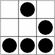
\includegraphics[width=0.5cm]{img/glider.png} }
\fancyfoot[RO]{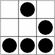
\includegraphics[width=0.5cm]{img/glider.png} \hfill
\textit{Comment devenir hacker // Alchimiste de l'informatique} \hfill \thepage}
\renewcommand{\headrulewidth}{0pt}
\renewcommand{\footrulewidth}{0.5pt}
\addtolength{\headheight}{0.5pt}
\fancypagestyle{plain}{
	\fancyhead{}
	\fancyfoot{}
	\renewcommand{\headrulewidth}{0pt}
}

%--- Definitions de nouvelles commandes ---
\newcommand{\N}{\mathbb{N}} % les entiers naturels


	\author{Gaby Wald}
	\title{Comment devenir hacker ? Alchimiste de l'informatique...}

%--- Pour le titre ---
\def\maketitle{%
	\begin{center}
		\begin{tabular}[c]{c p{0.3\textwidth}}
			\begin{tabular}{c}
				\textsc{\textbf{SENSO / REZO}}~\\[\baselineskip]~\\[\baselineskip]
				% \emph{\textbf{Dossier sp{\'e}cial}}~\\[\baselineskip]~\\[\baselineskip]
				\emph{\textbf{Documentation InterWeb}}~\\[\baselineskip]~\\[\baselineskip]
				\textsc{Gaby Wald}~\\[\baselineskip]~\\[\baselineskip]
			\end{tabular}
			& 
			\begin{tabular}{c}
				~\\[\baselineskip]
				~\\[\baselineskip]
				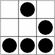
\includegraphics[width=3cm]{img/glider.png}~\\[\baselineskip]
			\end{tabular}
		\end{tabular}
		% \\ \hline
		 	% % if more than one logo
			% 
\includegraphics[width=5cm]{img/logo_glider.eps}
			% 
\includegraphics[width=5cm]{img/logo_wifi.eps}
		% \\ \hline
		% \end{tabular}
			~\\[\baselineskip]~\\[\baselineskip]
			\Huge{Comment devenir Hacker ?}~\\[\baselineskip]
			\Large{Alchimiste de l'informatique...}~\\[\baselineskip]
		
		~\\[\baselineskip]
		~\\[\baselineskip]
	\large{
		\textsc{\textbf{<<In Interweb We Trust>>}}
		~\\[\baselineskip]
		% <<titre personne>> : \texttt{Anne ONYME}~\\[\baselineskip]
		% <<titre personne>> : \texttt{Jocelyn CONNU}~\\[\baselineskip]
		~\\[\baselineskip]
		\textit{Re-Use and diffuse this documentation !}
	}

	\end{center}

}%



%--- Pour le glossaire --- a defaut de \makeglossary ou d'utilisation d'index latex

\definecolor{verylightgray}{rgb}{0.8,0.8,0.8}
\def\makeglossaire{%
	\begin{center}

	\begin{tabular}{|>{\columncolor{verylightgray}} p{0.2\textwidth}|p{0.8\textwidth}|}

		\hline

%		\textbf{BLAST} & 
%			\begin{tabular}{p{0.8\textwidth}}
%			Basic Local Alignment Search Tool \\
%			\textit{algorithmes et logiciels pour l'alignement de s{\'e}quences et la recherche de similarit{\'e}s locales}
%			\end{tabular} \\
%		\hline
		
		\textbf{AFNIC} & Association Fran\c{c}aise pour le Nommage Internet en Coop{\'e}ration \\

		\hline
		
		\textbf{DNS} & Domain Name Server \\

		\hline
		
		\textbf{FTP} & File Transfert Protocol \\

		\hline
		
		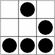
\includegraphics[width=1cm]{img/glider.png} & 

		\textbf{GLIDER} est le logo des hacker, symbole repris du jeu de la vie (cavalier ou planeur). \\
		
		\hline
		
		\textbf{HTML} & HyperText Markup Language \\

		\hline
		
		\textbf{HTTP} & 
			\begin{tabular}{p{0.8\textwidth}}
			HyperText Transfert Protocol \\
			\textit{Transfert des pages web. }
			\end{tabular} \\

		\hline
		
		\textbf{ICANN} & Internet Corporation for Assigned Names and Numbers \\

		\hline

		\textbf{NNTP} & News Network Transfert Protocol \\

		\hline
		
		\textbf{OS} & Operating System (\textit{Syst{\`e}me d'Exploitation}) \\

		\hline
		
		\textbf{RAM} & 
			\begin{tabular}{p{0.8\textwidth}}
			Random Access Memory (\textit{M{\'e}moire vive d'un ordinateur}) \\
			\textit{M{\'e}moire directement utilis{\'e}e et g{\'e}r{\'e}e par le processeur, plus rapide que le disque dur.  }
			\end{tabular} \\

		\hline
		
		\textbf{SMTP} & 
			\begin{tabular}{p{0.8\textwidth}}
			System of Mail Transfert Protocol \\
			\textit{Transfert des courriers {\'e}lectroniques. }
			\end{tabular} \\

		\hline

		\textbf{TCP / IP} & Transmission Control Protocol / Internet Protocol \\

		\hline
		
		\textbf{TOEFL} & Test Of English as a Foreign Language \\

		\hline
		
		\textbf{TOEIC} & Test Of English For International Communication \\

		\hline
		
		\textbf{URL / URI} & Universal Ressource Locator / Identifier \\

		\hline
		

		

	\end{tabular}

\end{center}

}%

%============================= Corps =================================
\begin{document}
	% pdftitle={Comment devenir hacker ? Alchimiste de l'informatique...}
	% pdfauthor={GabyWald}
	% pdfkeywords={hacker,alchimiste,information,programmation}
%ecrire le titre...
\maketitle
\setcounter{page}{0}
\thispagestyle{empty}
\clearpage

~\\
\setcounter{page}{0}
\thispagestyle{empty}
\clearpage

\setcounter{page}{1}

%% le contenu

% \rule{10cm}{0.5mm}~\\

\section*{Introduction\markboth{Introduction}{Introduction}}
\addcontentsline{toc}{section}{Introduction}

Les informations et conseils donn{\'e}s dans ce document r{\'e}sument le minimum {\`a} savoir en mati{\`e}re d'informatique et de culture hacker, pour plus de d{\'e}tails sur l'informatique et la culture hacker, voyez les sites et r{\'e}f{\'e}rences conseill{\'e}s {\`a} la fin du document. Voici d'abord les neuf points principaux et leur d{\'e}veloppement pour d{\'e}buter votre <<formation>> de hacker... La suite est l{\`a} pour vous aiguiller un peu plus au sein de la culture hacker.

% ecrire la table des mati{\`e}res, des figures et celle des tableaux
\tableofcontents

% \listoffigures
% ~\\ \rule{10cm}{0.5mm}~\\
% \listoftables
\clearpage

\part*{Les neufs points essentiels\markboth{Les neufs points essentiels}{Les neufs points essentiels}}
\addcontentsline{toc}{part}{Les neufs points essentiels}

\section{Apprendre {\`a} utiliser le r{\'e}seau}

	\subsection{Le fonctionnement du r{\'e}seau}
			L'acc{\`e}s {\`a} internet s'effectue {\`a} partir d'un ordinateur client vers un serveur (celui d'un Fournisseur d'Acc{\`e}s Internet, FAI, la plupart du temps). Ce serveur {\'e}tant connect{\'e} {\`a} de nombreux autres via les syst{\`e}mes de t{\'e}l{\'e}communication (cables sous-marin, satellites ou simples fils t{\'e}l{\'e}phoniques), c'est ce qui contitue un r{\'e}seau. Internet n'est que le terme d{\'e}signant l'ensemble de ces r{\'e}seaux interconnect{\'e}s entre eux. Le dialogue entre les diff{\'e}rents ordinateurs (clients et serveurs) est le protocole TCP/IP.

	\subsection{Le protocole d'internet : TCP/IP}
			
			TCP/IP est le protocole d'usage d'internet (celui qui permet de connecter les ordinateurs entre eux), les {\'e}changes entre ordinateurs s'effectue gr{\^a}ce {\`a} des adresses du type xxx.xxx.xxx.xxx (pour IP4) avec xxx compris entre 0 et 255. Il y a des adresses r{\'e}serv{\'e}es, ex : 127.0.0.1 d{\'e}signe toujours l'ordinateur local, et 192.168.xxx.xxx ou 10.xxx.xxx.xxx des adresses de r{\'e}seaux locaux ou intranet (adresses IP r{\'e}serv{\'e}es {\`a} cet usage et non utilis{\'e}es sur internet c'est {\`a} dire non accessible directement par l'ext{\'e}rieur du r{\'e}seau intranet).~\\

			Une adresse IP indique un ordinateur particulier sur le r{\'e}seau, de plus le m{\'e}canisme des ports r{\'e}seaux permet d'indiquer quel programme doit traiter les informations passant d'un ordinateur {\`a} l'autre (chaque <<sous-protocole>>, voir paragraphe suivant, a un port sp{\'e}cifique : courrier, page web...). ~\\

			L'adresse IP peut {\^e}tre remplac{\'e}e par un nom de domaine (nom et suffixe comme .com .fr .biz) ; des serveurs appel{\'e}s DNS (Domain Name Servers) sont charg{\'e}s d'{\'e}tablir la correspondance nom/IP {\`a} la demande d'autres serveurs car si l'on donne le nom {\`a} son navigateur internet, l'adresse IP est n{\'e}cessaire pour la communication et l'{\'e}change entre les ordinateurs (et cela se fait de fa\c{c}on transparente). La r{\'e}gulation des noms de domaine et leur attribution est effectu{\'e}e par des organismes internationaux comme l'Afnic en France (Association Fran\c{c}aise pour le Nommage Internet en Coop{\'e}ration, $<$\emph{http://www.afnic.fr/}$>$ ) ou l'ICANN (Internet Corporation for Assigned Names and Numbers).

	\subsection{Le syst{\`e}me Client/serveur}

			Un serveur est un ordinateur puissant (en termes de puissance de calcul, de stockage et d'entr{\'e}e-sorties) founissant en services (pages web, courrier {\'e}lectronique, news, fichier, connexion...). Un ordinateur personnel est un exemple de client. L'avantage d'un tel syst{\`e}me est que l'ordinateur client ne voit que le serveur (il doit passer par lui pour acc{\'e}der au reste du r{\'e}seau) par le biais de ses programmes qui r{\'e}cup{\`e}rent et traitent les informations envoy{\'e}es par le serveur. ~\\

			Un ordinateur client s'adresse {\`a} l'ordinateur serveur par le biais des protocoles et des ports qui leurs sont attribu{\'e}s, le serveur r{\'e}ponde de la m{\^e}me fa\c{c}on au client avec les informations que celui-ci demande (ou une erreur le cas {\'e}ch{\'e}ant). Ce syst{\`e}me a plusieurs avantages, administr{\'e} et s{\'e}curis{\'e} de fa\c{c}on centralis{\'e}e, le r{\'e}seau {\'e}volut ainsi sans avoir {\`a} changer tous les clients. Mais le serveur est aussi le point faible du r{\'e}seau (en plus de son prix) car il constitue un noeud du r{\'e}seau. ~\\

	\subsection{Les navigateurs internet (adresses types : http, https, ftp,...)}

			Un navigateur internet est un logiciel qui permet d'afficher les pages des sites internet et de naviguer entre ces pages via les liens hypertextes; Les pages sont cod{\'e}es en HTML (HyperText Markup Language) : langage de programmation traduit par le navigateur. Ce langage fonctionne gr{\^a}ce {\`a} des balises de style encadrant le texte dont le style est {\`a} modifier (en gras, italique, soulign{\'e}...) ou renvoyant des informations particuli{\`e}res (balises des liens hypertextes, qui renvoient vers d'autres pages, affichage d'une image...). ~\\

		Par exemple dans une page re\c{c}ue par votre navigateur <b>texte en gras</b> sera affich{\'e} de cette fa\c{c}on par votre navigateur : \textbf{texte en gras} ; <i>texte en italique</i> deviens \textit{texte en italique}. Ceci s'effectue comme dans un traitement de texte, sauf que les pages peuvent seulement {\^e}tre consult{\'e}es sur le site. ~\\

		Un lien hypertexte est donc un mot, une expression ou une phrase encadr{\'e}e par une balise contenant l'adresse de la page suivante auquel l'expression renvoie. L'adresse (ou URL pour Universal Ressource Locator) est cod{\'e} de la fa\c{c}on suivante : $<$\emph{http://www.serveur.com/repertoire/page.html}$>$ o{\`u} <<http://>> est l'un des protocoles vus au point 7, <<www.serveur.com>> est l'adresse du serveur contenant la page et <<repertoire/page.html>> est le chemin d'acc{\`e}s {\`a} la page sur le serveur. ~\\

		L'{\'e}criture de l'adresse dans la barre du navigateur ou le clic sur un lien indique au navigateur d'acc{\'e}der {\`a} la page concern{\'e}e (si elle existe), et le navigateur s'occuper du reste (demande de la page via les protocoles TCP/IP et http gr{\^a}ce {\`a} l'ordinateur) et traduction lisible de la page (traduction des balises en apparence du texte). ~\\

		Il existe diff{\'e}rents navigateurs internets : FireFox, Mozilla, Safari, Internet Explorer (fr{\'e}quent mais peu performant...). Ils ont tous des capacit{\'e}s similaires, certains sites internets {\'e}tant plus adapt{\'e}s {\`a} certains (ou pas du tout adapt{\'e}s). ~\\~\\~\\

	\subsection{Le courrier {\'e}lectronique}
\textit{(adresses du type prenom.nom@fournisseur.com ou surnom@serveur.fr)}

			Les adresses de courrier {\'e}lectroniques sont diff{\'e}rentes des adresses utilis{\'e}es par un navigateur, notamment par la pr{\'e}sence de l'arobase (symbole a enroul{\'e} ou @ - arobase). Leur signification est simple : elles comportent un nom (une personne en g{\'e}n{\'e}ral) et le nom du serveur contenant une boite de courrier pour cette personne. ~\\

			Le courrier {\'e}lectronique permet, comme le courrier traditionnel, l'{\'e}change d'informations textuelles, d'images ou de fichiers (en pi{\`e}ces jointes)... De plus, un m{\^e}me message peut {\^e}tre exp{\'e}di{\'e} {\`a} plusieurs adresses en m{\^e}me temps (le serveur d'envoi du courrier s'occupant ensuite de faire une copie pour chaque destinataire). {\'e}videmment, certains {\'e}l{\'e}ments sont tr{\`e}s proches du courrier traditionnel : on peut demander un accus{\'e} de r{\'e}ception (l'ordinateur de r{\'e}ception se charge de vous l'envoyer si vous en demandez un), et si votre correspondant n'existe pas ou plus, le courrier revient...~\\

	\subsection{Les newsgroups (news:)}
			Les news servent {\`a} {\'e}changer des informations sur des th{\`e}mes pr{\'e}cis et class{\'e}s, auquels il est possible de s'abonner via usenet ou les groupes googles, ainsi que de nombreux autres sites qui le proposent. Certains logiciels permettent d'acc{\'e}der directement sans passer par les sites d{\'e}di{\'e}s mais peuvent passer par un abonnement (via votre fournisseur d'acc{\`e}s {\`a} internet). Chaque groupe de news poss{\`e}de une ambiance sp{\'e}cifique et ses habitu{\'e}s, prenez soin de lire les diff{\'e}rents sujets en cours, la Foire Aux Questions (FAQ), la pr{\'e}sentation du groupe... afin de vous faire une id{\'e}e assez pr{\'e}cise des sujets abord{\'e}s et de la personnalit{\'e} des habitu{\'e}s. ~\\

			Des r{\^e}gles de politesse existent sur ces forum, pour les plus {\'e}videntes il s'agit surtout de ne pas poster <<hors sujet>>, {\'e}viter d'envoyer des propos injurieux ou de poser une question en {\'e}crivant que l'on ne viendra pas lire les r{\'e}ponses... Une Foire Aux Question et une pr{\'e}sentation du groupe sont post{\'e}s r{\'e}guli{\`e}rement, tous les quinze jours ou tous les mois ; lisez attentivement ces documents afin d'{\'e}viter les erreurs...~\\


\section{Apprendre {\`a} lire (et {\`a} {\'e}crire) en anglais}
		\c{C}a, on est cens{\'e} le faire {\`a} l'{\'e}cole, mais le faire de soi-m{\^e}me et se maintenir au top niveau c'est mieux ! Lire des livres en anglais est une bonne solution pour y arriver, une visite {\`a} la biblioth{\`e}que la plus proche est une fa\c{c}on de trouver des livres en anglais (ou dans une librairie). ~\\

	L'anglais est devenue une langue internationale, mal pratiqu{\'e}e {\`a} peu pr{\`e}s partout dans le monde, mais malgr{\'e} tout utile pour l'{\'e}change d'informations et de donn{\'e}es. {\`a} moins de trouver une autre langue d'{\'e}change avec un correspondant ou pour rechercher une information. ~\\

	Quelques adresses internet : 
	\begin{itemize}
		\item $<$\emph{http://www.anglaisfacile.com/}$>$
		\item $<$\emph{http://www.e-anglais.com/}$>$
	\end{itemize}~\\

	Un bon conseil est de passer le test TOEIC (Test Of English For International Communication) ou TOEFL (Test Of English as a foreign language), \c{c}a fait toujours bien sur le Curriculum Vitae... Et l'anglais est (malheureusement ?) utile partout : autant pour le travail qu'{\`a} titre personnel, les notices techniques, certaines informations ne sont disponibles qu'en anglais (donn{\'e}es scientifiques et informatiques)...~\\

\section{D{\'e}couvrez comment marche votre ordinateur}
		La carte m{\`e}re rassemble les {\'e}l{\'e}ments principaux pour un bon fonctionnement de l'ordinateur et s'occupe du traitement et de l'{\'e}change de donn{\'e}es avec les autres {\'e}l{\'e}ments de l'ordinateur ({\'e}cran, disques, p{\'e}riph{\'e}riques divers). Le processeur est l'unit{\'e} de calcul centrale, li{\'e}e {\`a} diff{\'e}rents registres de calculs inclus et {\`a} la m{\'e}moire vive (RAM). D'autres {\'e}l{\'e}ments peuvent s'ajouter {\`a} la carte m{\`e}re, essentiellement des <<cartes filles>> : carte son, carte vid{\'e}o, carte Ethernet... Ces derni{\`e}res permettent d'acc{\'e}l{\'e}rer ou de remplir certaines fonctions en plus du processeur de la carte m{\`e}re car ils comportent des processeurs d{\'e}di{\'e}s {\`a} des algorithmes de calculs particuliers, ainsi que des connections particuli{\`e}res vers d'autres {\'e}l{\'e}ments. ~\\

		Le disque dur est une superposition de disques magn{\'e}tiques avec un <<rateau>> de t{\^e}tes de lectures dans une boite scell{\'e}e. Il est organis{\'e} en cercles concentriques divis{\'e}s en secteurs. Le premier secteur (dit de <<d{\'e}marrage>>) contient toutes les informations sur l'organisation du disque dur (num{\'e}rotation en s{\'e}quence...), cette organisation d{\'e}pend essentiellement du syst{\`e}me de fichier, ce dernier {\'e}tant g{\'e}n{\'e}ralement sp{\'e}cifique {\`a} chaque syst{\`e}me d'exploitation (ext2, UFS, VFS, VFAT, NTFS, HFS...). Certains syst{\`e}mes tol{\'e}rant plusieurs syst{\`e}mes de fichiers, voire plusieurs disques et partitions de disques (c'est le cas de la plupart des syst{\`e}mes actuellement). ~\\

		La communication entre les diff{\'e}rents {\'e}l{\'e}ments s'effectue gr{\^a}ce aux mappes de connexion, ce sont des regroupements de fils, chacun sp{\'e}cifique d'un type de circuit. Entre deux {\'e}l{\'e}ments (carte m{\`e}re et disque dur par exemple), une mappe compl{\`e}te permet un transfert rapide de plusieurs informations en m{\^e}me temps : commandes de l'un, r{\'e}ponses de l'autre, transfert de donn{\'e}es... 

		Le clavier et la souris sont les principaux p{\'e}riph{\'e}riques d'entr{\'e}es de l'utilisateur vers l'ordinateur. Le clavier permet d'entr{\'e}es des donn{\'e}es textuelles aphanum{\'e}riques et d'envoyer des commandes (lignes de commandes ou combinaison de touches avec <<control>> par exemple), le clavier envoie comme information les coordonn{\'e}es de la touche (que le syst{\`e}me d'exploitation traduit). La souris permet la s{\'e}lection et la commande d'{\'e}l{\'e}ments au sein d'une interface graphique (menus, fen{\^e}tres, ic{\^o}nes), la souris peut exister sous diff{\'e}rentes formes depuis la forme classique (boule et barres rotatives) {\`a} la souris <<laser>> en passant par la <<sph{\`e}re pos{\'e}e>> ou le stylet, l'essentiel du fonctionnement de la souris se limite {\`a} la transmission du mouvement et des pressions sur le ou les bouttons, le syst{\`e}me d'exploitation s'occupe ensuite de transformer l'information en changement de coordonn{\'e}es ou lancement de fonctions particuli{\`e}res. ~\\

	L'ordinateur ne peut vraiment fonctionner qu'avec un syst{\`e}me d'exploitation. C'est un logiciel charg{\'e} de g{\'e}rer l'ensemble des composants de l'ordinateur : processus en cours sur le processeur, gestion de la m{\'e}moire (m{\'e}moire vive et disque dur), gestion des entr{\'e}es / sorties (clavier, souris... et affichage {\`a} l'{\'e}cran !). ~\\

	Diff{\'e}rents syst{\`e}mes d'exploitations existent : Unix (ancien, robuste et encore tr{\`e}s utilis{\'e}), Windows (depuis 1995), Mac OS (depuis 1984), Linux, BeOS... Tous disposent d'avantages (et parfois d'inconv{\'e}nients), mais ils ont en actuellement des interfaces graphiques performantes toutes tr{\`e}s proches les unes des autres. 

\section{S'amuser {\`a} r{\'e}soudre des probl{\`e}mes}
		Participez {\`a} des exercices de cryptographie, des chasses au tr{\'e}sor, ou des r{\'e}solutions d'{\'e}nigmes, une simple recherche sur internet suffit via votre moteur de recherche favori avec les termes <<cryptographie>>, <<chasse au tr{\'e}sor>>... Un exemple idiot pour favoriser la r{\'e}flexion : chercher un document dans une voire plusieurs biblioth{\`e}ques (municipales, universitaires, centres de documentation) et noter la fa\c{c}on dont ils sont tri{\'e}s et rang{\'e}s. ~\\

		Un autre exemple : s'amuser {\`a} des exercices de codage et de d{\'e}codage en diff{\'e}r{\'e} (plusieurs semaines ou mois entre les deux en <<perdant>> la solution de retour au texte de d{\'e}part) en solitaire ou avec des amis, on peut tester ainsi diff{\'e}rents syst{\`e}mes de codages manuels ou {\'e}lectroniques...~\\

		Le meilleur exemple de r{\'e}solution de probl{\`e}me que l'on puisse donner sur ordinateur est... un jeu vid{\'e}o ! Il s'agit du jeu <<Myst>> et de ses suites (Riven, Exile, Revelation, Uru...). L'{\'e}tat d'esprit est effectivement celui de la r{\'e}solution d'enigmes sans avoir besoin de pirater le jeu dans tous les sens du terme (pas de t{\'e}l{\'e}chargement ill{\'e}gal ou de <<d{\'e}plombage>>) : un papier, un crayon et un peu de r{\'e}flexion s'imposent (en plus de l'ordinateur et du jeu). ~\\

\section{Apprendre {\`a} programmer}
		Au moins un langage de programmation, si possible orient{\'e} objet. Un langage de programmation permet de faire executer des t{\^a}ches (souvent r{\'e}p{\'e}titives) par un ordinateur au travers d'un programme cod{\'e} dans un langage compr{\'e}hensible par l'ordinateur. La notion d'objet en programmation informatique correspond {\`a} une entit{\'e} manipulable au sein du programme mais distincte des variables et des donn{\'e}es, un objet est caract{\'e}ris{\'e} par des attributs (variables) des m{\'e}thodes (fonctions et op{\'e}rations sp{\'e}cifiques {\`a} cet objet). ~\\

		Pour apprendre la programmation (et l'algorithmique pour la conception de programmes), vous pouvez voir le langage Scheme pour les bases (d{\'e}finir variables, facilement mettre en oeuvre un algorithme, notion d'objet avec le lambda calcul), ce langage de programmation est de la famille des LISP. Pour continuer avec d'autres langages de programmation voyez aussi Java (assez universel car il permet d'appr{\'e}hender directement <<l'orient{\'e} objet>>). Pour continuer, il existe aussi C/C++, Python...~\\

\section{{\'E}tudier les syst{\`e}mes de s{\'e}curit{\'e} et de cryptographie}
		Les syst{\`e}mes se s{\'e}curit{\'e} en informatique concernent essentiellement la lutte contre les virus informatiques et les attaques de syst{\`e}mes informatique (acc{\`e}s par le r{\'e}seau ou non). Pour assurer la s{\'e}curit{\'e} d'un ordinateur, de nombreux syst{\`e}mes existent, suffisement fiables si ils sont configur{\'e}s correctement voire renouvel{\'e}s r{\'e}guli{\`e}rement : anti-virus (d{\'e}tection et suppression des programmes dangereux pour l'ordinateur voire pour l'utilisateur), mot de passe et firewall (emp{\^e}cher l'acc{\`e}s {\`a} l'ordinateur de fa\c{c}on anormale), cryptographie (encodage de l'information)...~\\

		{\'E}tudier ces syst{\`e}mes est une continuit{\'e} de la r{\'e}solution d'{\'e}nigmes et de la r{\'e}solution de probl{\`e}mes. Cela permet aussi de mieux comprendre comment marche le r{\'e}seau et les algorithmes de chiffrement (tr{\`e}s utile de comprendre les algorithmes dans les programmes...). Sans pour autant utiliser ces connaissances pour contourner ces syst{\`e}mes, elles sont utiles pour lutter contre les virus, les <<acteurs ill{\'e}gaux>> et les petits marrants...~\\

\clearpage

\section{Apprenez {\`a} conna{\^i}tre les protocoles de r{\'e}seaux}
		Des protocoles sont utilis{\'e}s par le biais du TCP/IP (ils passent par ce dernier de fa\c{c}on transparente) : 
\begin{itemize}
	\item <<http>> est l'abr{\'e}viation de <<HyperText Transfert Protocol>> ou transfert de protocole hypertexte (en fran\c{c}ais), ce protocole sert au tranfert des fichiers internets (pages web) du WWW (World Wide Web ou toile d'araign{\'e}e mondiale). <<https>> en est la version s{\'e}curis{\'e}e, pour les sites web n{\'e}cessitant un {\'e}change crypt{\'e} comme les sites marchands. 
	\item <<ftp>> d{\'e}signe le <<File Transfert Protocol>> ou protocole d'{\'e}change de fichier. Ce protocole permet le t{\'e}l{\'e}chargement de fichier (des logiciels par exemples) sans forc{\'e}ment passer par un navigateur. 
	\item L'acc{\`e}s au courrier {\'e}lectronique (e-mail) passe par les protocoles POP (Post Office Protocole) et IMAP (Internet Mail Advanced Protocol) quand votre ordinateur se connecte au serveur pour r{\'e}cup{\'e}rer le courrier {\'e}lectronique. Le protocole SMTP (Simple Mail Transfert Protocol) est le protocole de transfert du courrier de serveurs {\`a} sevreurs ou de votre ordinateur au serveur, ce protocole permet l'acheminement du courrier vers son destinataire. 
	\item L'acc{\`e}s aux serveurs de news utilise le protocole NNTP, Network News Transport Protocol. Que ce soit par un navigateur internet ou un logiciel d{\'e}di{\'e} (lecteur de news), ce protocole est l'un des plus utiles d'internet car il permet la transmission de messages sur un th{\`e}me particulier de serveurs {\`a} serveurs. Voyez Usenet pour plus d'informations : $<$\emph{http://www.usenet-fr.net/}$>$. 
	\item L'IRC (Instant Relay Chat) est un protocole qui permet {\`a} des personnes distantes g{\'e}ographiquement de communiquer, sous la forme de chat. La grande particularit{\'e} de l'IRC est qu'il <<enregistre>> toutes les conversations sous la forme de logs. Dans les communaut{\'e}s de d{\'e}veloppement Open Source, cet outil est d'une importance majeure en ce qu'il permet aux d{\'e}veloppeurs d'{\^e}tre en liaison de fa\c{c}on continue, et d'avoir acc{\`e}s {\`a} ce qui s'est {\'e}crit pendant leur absence.
\end{itemize}~\\

	Comme indiqu{\'e} plus haut, chaque protocole passe par un port particulier, par exemple le port 80 pour le protocole http, 25 pour SMTP, 110 pour POP, 443 pour https, 6667 pour IRC... Cela permet un traitement particulier par le syst{\`e}me d'exploitation et les logiciels qui utilisent ces protocoles (ces ports peuvent {\^e}tre modifi{\'e}s  par l'utilisateur, mais par convention, ce sont ceux utilis{\'e}s par d{\'e}faut).~\\

\clearpage

\section{Utiliser un syst{\`e}me Unix open source : LINUX, BSD...}
		Pourquoi utiliser Linux ? Pour changer de votre syst{\`e}me d'exploitation habituel (on peut raisonnablement penser qu'il s'agit de windows) et vous apprendre un syst{\`e}me qui utilise des normes assez standards et universelles (syst{\`e}mes unix et assimil{\'e}s dans les universit{\'e}s et les entreprises, syst{\`e}mes analogues, Mac OS X). On trouve maintenant de tr{\`e}s belles interfaces graphiques solides (Gnome et KDE par exemple) en plus du syst{\`e}me de ligne de commande tr{\`e}s formateur pour comprendre le fonctionnement d'un syst{\`e}me d'exploitation...~\\

		Faciles {\`a} installer, on trouve Linux en grande surface : Suse, Mandrake... Sans compter les manuels tr{\`e}s bien faits, faciles {\`a} trouver dans les librairies sp{\'e}cialis{\'e}es (et aussi g{\'e}n{\'e}ralistes), un livre comme <<Linux pour les nuls>> est excellent pour commencer, et cela compl{\`e}tera tr{\`e}s bien ce document, ainsi que certains magazines informatiques plus ou moins sp{\'e}cialis{\'e}s qui fournissent parfois un linux complet sur un disque (CD ou DVD g{\'e}n{\'e}ralement).~\\

		Ubuntu est un syst{\`e}me d'exploitation Linux qui peut {\^e}tre t{\'e}l{\'e}charg{\'e} gratuitement ou envoy{\'e} gratuitement sur CD par voie postale via une demande sur $<$\emph{https://shipit.ubuntu.com/}$>$, tr{\`e}s facile {\`a} installer sur tout ordinateur, il suffit de se laisser guider  ; petite surprise : on peut {\'e}galement d{\'e}marrer un ordinateur avec ce CD, tout comme avec les Live-CD Knoppix et d{\'e}riv{\'e}s. ~\\

\section{Restez loin des outils d'attaques ou ill{\'e}gaux}
		{\`A} quoi sert un mailbomber ? Faire du spam, donc {\`a} encombrer le r{\'e}seau (les services de courrier {\'e}lectroniques ont, de toute fa\c{c}on, tendance {\`a} effacer directement les messages r{\'e}p{\'e}t{\'e}s plus de cinq ou dix fois). {\`a} quoi cela peut-il servir d'effacer (ou tenter d'effacer) le disque dur d'une personne que vous venez {\`a} peine de rentrer sur IRC ou chat ? Rien, sinon vous faire exclure... ~\\

		Aimeriez-vous que votre ordinateur subissent les cons{\'e}quences d'une telle attaque en r{\'e}ponse {\`a} un tel comportement ? Je crois que non, surtout si la personne en face est plus comp{\'e}tente que vous (si c'est le cas, oubliez votre pare-feu / firewall et votre antivirus)... J'esp{\`e}re que vous aurez compris pourquoi ne pas utiliser ces logiciels g{\'e}n{\'e}ralement ill{\'e}gaux... Si vous n'avez pas encore compris, m{\'e}ditez : <<Taper sur les autres pour montrer que l'on est le meilleur... est la meilleure fa\c{c}on de montrer que l'on est un imb{\'e}cile. >> (si les terroristes pensaient {\`a} \c{c}a, on serait plus tranquilles). ~\\

\clearpage
% \rule{10cm}{0.5mm}~\\

Voil{\`a} donc pour les neufs points essentiels, que l'on peut d{\'e}velopper tr{\`e}s fortement par les {\'e}l{\'e}ments qui suivent dans les pages suivantes, mais {\^e}tre hacker, c'est aussi savoir chercher des informations compl{\'e}mentaires sans point de vue <<pr{\^e}t {\`a} l'emploi>>. ~\\

% \clearpage

\rule{10cm}{1mm}~\\

\section*{Conseils suppl{\'e}mentaires\markboth{Conseils suppl{\'e}mentaires}{Conseils suppl{\'e}mentaires}}
\addcontentsline{toc}{part}{Conseils suppl{\'e}mentaires}

Pour devenir un hacker, \textbf{r{\'e}p{\'e}tez les phrases suivantes} jusqu'{\`a} y croire r{\'e}ellement : 
\begin{enumerate}
\item Le monde est plein de probl{\`e}mes fascinants qui n'attendent que d'{\^e}tre r{\'e}solu. 
\item Personne ne devrait jamais avoir {\`a} r{\'e}soudre le m{\^e}me probl{\`e}me deux fois.
\item La routine et l'ennui sont inacceptables. 
\item Vive la libert{\'e}!
\item L'attitude n'est pas un substitut {\`a} la comp{\'e}tence. Pour cela il vous faut : ~\\
	\begin{enumerate}
	\item Apprendre {\`a} programmer. 
	\item Installer un Unix libre et apprendre {\`a} s'en servir.
	\item Apprendre {\`a} utiliser le World Wide Web et {\`a} {\'e}crire en HTML. 
	\end{enumerate}
\end{enumerate}~\\


Les statuts dans la culture des hackers sont principalement socio-culturels selon vos centres d'int{\'e}r{\^e}t et votre aptitude {\`a} communiquer avec d'autres (geek, nerd...). Il y a principalement cinq types de \textbf{choses {\`a} faire pour {\^e}tre respect{\'e}} par les hackers : 
\begin{enumerate}
	\item {\'E}crire des logiciels libres. 
	\item Aider {\`a} tester et {\`a} d{\'e}bugger des logiciels libres. 
	\item Publier des informations utiles. 
	\item Aider {\`a} faire tourner l'infrastructure
	\item Servir la culture des hackers elle-m{\^e}me.
\end{enumerate}~\\

\rule{10cm}{0.5mm}~\\

Encore une fois, pour {\^e}tre un hacker, il faut entrer dans l'{\'e}tat d'esprit du hacker. Pour cela, il y a quelques activit{\'e}s que l'on pratique loin d'un ordinateur qui semblent aider. Ce ne sont {\'e}videmment pas des substituts {\`a} la pratique de l'informatique, mais de nombreux hackers les pratiquent, et pensent qu'elles sont reli{\'e}es de fa\c{c}on fondamentale {\`a} l'essence du hack.~\\

% \rule{10cm}{0.5mm}~\\

Une liste de \textbf{choses {\`a} faire} pour \textbf{compl{\'e}ter votre <<Hacker Attitude>>} (et {\^e}tre d{\'e}finitivement un geek, ou un nerd si vous {\^e}tes vraiment asocial) : 
\begin{itemize}
	\item Lire de la science-fiction. Aller {\`a} des conventions de SF (un bon moyen pour rencontrer des hackers et des proto-hackers). 
	\item Pratiquer le Zen et/ou les arts martiaux (pour la discipline mentale). 
	\item {\'E}couter et analyser de la musique, apprendre {\`a} appr{\'e}cier des formes particuli{\`e}res de musique. Apprendre {\`a} bien jouer d'un instrument, ou {\`a} chanter. 
	\item Appr{\'e}cier les jeux de mots. 
	\item Apprendre {\`a} bien {\'e}crire dans sa langue maternelle. 
\end{itemize}~\\

Une liste de \textbf{choses {\`a} \underline{ne pas} faire} (l'exclusion est g{\'e}n{\'e}ralement rapide quand cela arrive, m{\^e}me involontairement)
\begin{itemize}
	\item Ne pas utiliser des noms de login grandiloquents ou stupides. 
	\item Ne pas intervenir dans les flame wars [guerres au lance-flamme] dans les  newsgroups Usenet ou ailleurs. 
	\item Ne pas s'autoproclamer <<cyberpunk>>, et ne pas perdre son temps avec quelqu'un qui le fait. 
	\item Ne pas poster de message rempli de fautes d'orthographe ou de grammaire. 
\end{itemize}


\clearpage

\part*{Pour aller plus loin...\markboth{Pour aller plus loin...}{Pour aller plus loin...}}
\addcontentsline{toc}{part}{Pour aller plus loin...}

Adresses utiles
\begin{itemize}
	\item[$<$\emph{http://www.commentcamarche.net/}$>$] Cours d'informatique en ligne
	\item[$<$\emph{http://www.renater.fr/Projets/ICANN/}$>$] (en fran\c{c}ais sur l'ICANN)
	\item[$<$\emph{http://www.internic.net/}$>$] Site de l'InterNIC
	\item[$<$\emph{http://www.usenet-fr.net/}$>$] Utilisation de Usenet (en fran\c{c}ais)
	\item[$<$\emph{http://fr.wikipedia.org/}$>$] (encyclop{\'e}die Wikipedia en Fran\c{c}ais)
	\item[$<$\emph{http://fr.wikipedia.org/wiki/Cyberpunk}$>$] Pour l'article Cyberpunk
	\item[$<$\emph{http://fr.wikipedia.org/wiki/Hacker}$>$] Pour l'article Hacker
	\item[$<$\emph{http://fr.wikipedia.org/wiki/Cracker}$>$] Pour l'article Cracker
	\item[$<$\emph{http://fr.wikipedia.org/wiki/Geek}$>$] Pour l'article Geek
	\item[$<$\emph{http://fr.wikipedia.org/wiki/Nerd}$>$] Pour l'article Nerd
	\item 
	\item[$<$\emph{http://www.secuser.com/}$>$] Secuser, s{\'e}curit{\'e} informatique
	\item[$<$\emph{http://www.zataz.com/}$>$] Zataz Magazine
	\item 
	\item[$<$\emph{http://www.2600fr.org/}$>$] Les meetings 2600 en France
	\item[$<$\emph{http://hackerspaces.org/}$>$] Hacker Spaces Wiki
	\item[$<$\emph{http://www.tmplab.org/}$>$] /tmp/lab : Hacker Space fran\c{c}ais
\end{itemize}~\\

Pour information les termes Hacker et Cracker sont (presques) mutuellement exclusifs : l'un est un bidouilleur dans l'{\^a}me, l'autre veut d{\'e}truire ;  la mentalit{\'e} Geek est tr{\`e}s proche (voire d{\'e}finis) la mentalit{\'e} Hacker, un Nerd voire un Otaku est la version plus obscure du Geek...~\\





Quelques livres de science-fiction pour parfaire votre culture sont indiqu{\'e}s dans les r{\'e}f{\'e}rences bibliographiques...
\begin{itemize}
	\item L'ensemble des livres de William Gibson : \emph{Neuromancien}, \emph{Comte Z{\'ero}}...
	\item \emph{Cabl{\'e}}, \emph{Aristo{\"\i}} (Walter John Williams)
	\item \emph{Les mailles du r{\'e}seau} (Bruce Sterling)
	\item \emph{Les synth{\'e}r{\'e}tiques} (Pat Cadigan)
	\item La s{\'e}rie \emph{F.A.U.S.T.} (Serge Lehman)
	\item \emph{La reine des anges} (Greg Bear)
	\item \emph{Le Samoura{\"\i} Virtuel} (Neal Stephenson)
	\item \emph{Blade Runner} (Philip K. Dick)
	\item [...]
\end{itemize}


\clearpage

\section*{Abbr{\'e}viations\markboth{Abbr{\'e}viations}{Abbr{\'e}viations}}

\addcontentsline{toc}{section}{Abbr{\'e}viations}

%% voir en haut : sous la definition du titre : glossaire

\makeglossaire

\clearpage

\section*{Bibliographie\markboth{Bibliographie}{Bibliographie}}

\addcontentsline{toc}{section}{Bibliographie}
\nocite{*}
%toutes references biblio : 6 lettres + 2 chiffres
\bibliography{devenirhacker}
\bibliographystyle{frplain} % plain or frplain
\end{document}